\chapter[Implementação]{Implementação}

\section{Estrutura}

Para a realização de teste quanto ao tipo de motor será utilizado e para testes com a 
ponte H, foi construído de maneira rudimentar um protótipo.

O protótipo foi construído utilizando:
\begin{itemize}
	\item madeira;
	\item 4 rodas;
	\item 2 motores;
\end{itemize}

Inicialmente foram realizados testes utilizando dois motores DC fabricante HP, no entanto o uso destes foi descartado, pois se
tratavam de motores de velocidade e não apresentavam um torque mínimo solicitado no projeto. Buscando viabilizar o uso destes motores,
tentou-se a construção de uma caixa de engrenagem utilizando madeira e duas engrenagens em cada caixa, no entanto o eixo que fazia a
ligação do motor com estas gerou bastante atrito inviabilizando o uso destas, bem como o uso destes motores.

\begin{figure}[H]
    \centering
    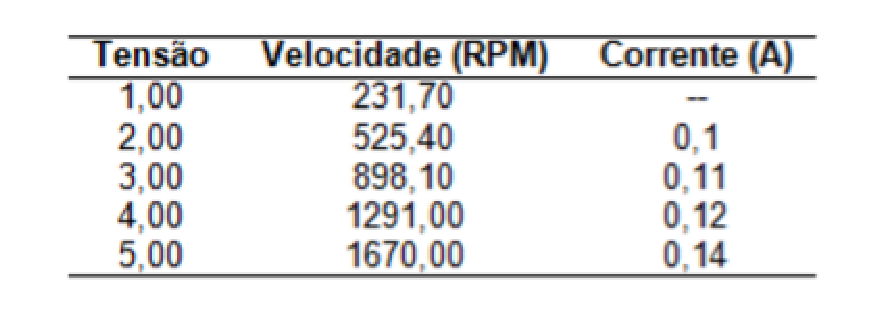
\includegraphics[width=1\textwidth]{figuras/tensao_vel.eps}
    \caption{Velocidade x Tensão do motor do 1ºTeste.}
    \label{fig:tensao_vel}
\end{figure}

O segundo teste foi realizado com motores reciclados de carrinhos de brinquedo, com isso não tínhamos as especificações deste.
Este motor foi descartado uma vez que em testes realizados no Laboratório NEI, na FGA este estava demandando uma corrente 3,3 A,
ou seja, estava demandando praticamente toda a corrente que o Raspberry PI tem para suprir todo o sistema, o teste com estes motores
mostrou que estes operam a vazio, mas quando se colocava uma carga neste, ele não tinha torque suficiente para girar.

O terceiro teste foi realizado com motores DC 3-6V, com caixa de redução e eixo duplo. Os testes realizados com os dois motores deste
protótipo necessitavam de 3,3V e a corrente demanda pelos dois oscilava entre 0,5 e 0,6 A. Se verificou a movimentação geral do robô,
nos sentidos para frente e para trás, atentando-se aos limites de tensão e corrente. Depois se verificou a desempenho geral da curva do
robô, sendo realizada por diferença de rotação nos dois motores.

\begin{figure}[H]
    \centering
    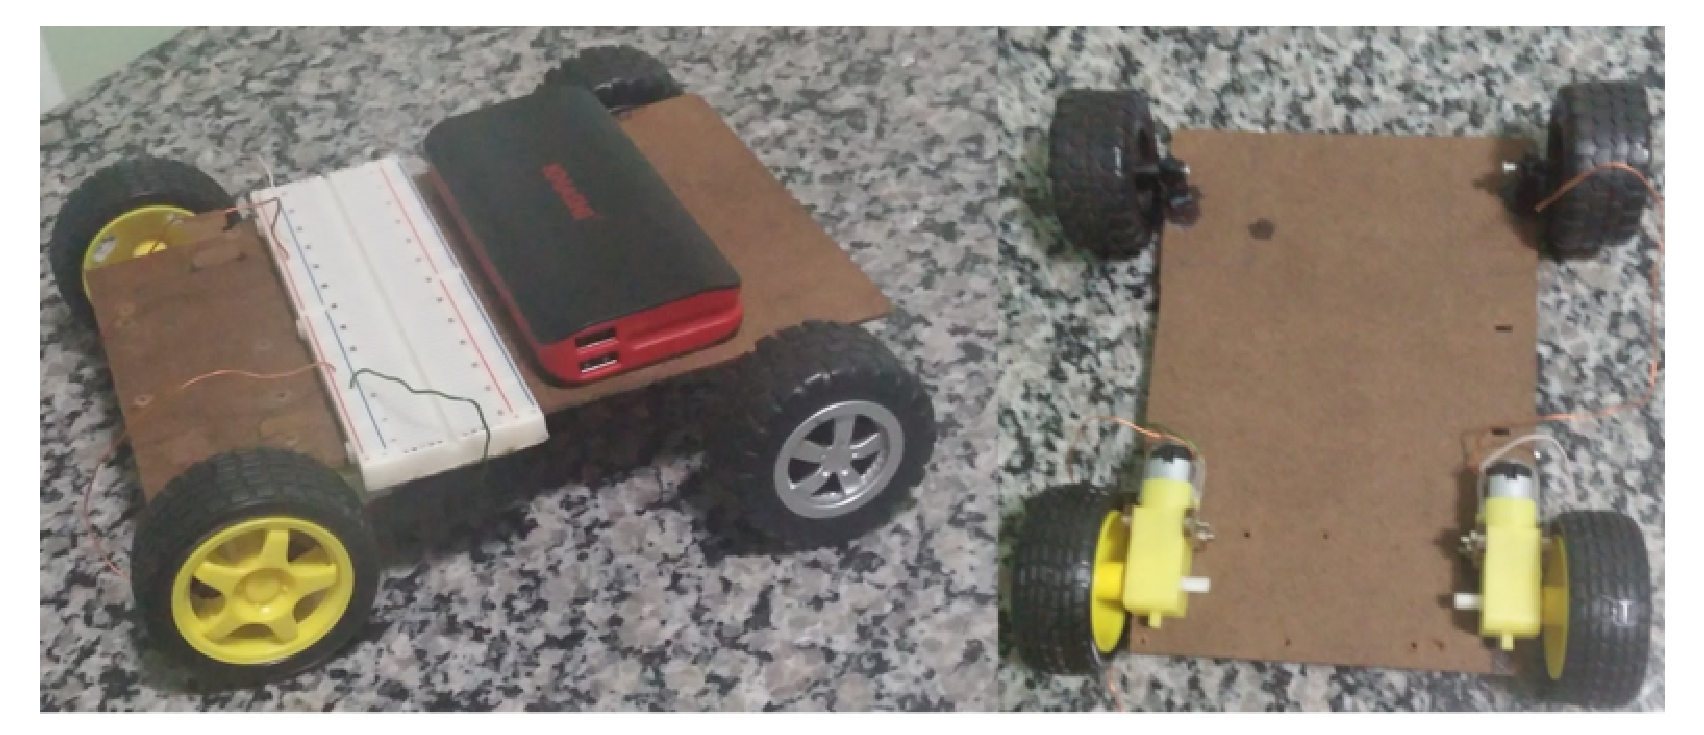
\includegraphics[width=1\textwidth]{figuras/prototipo_01.eps}
    \caption{Protótipo preliminar do robô Alfa.}
    \label{fig:prototipo_01}
\end{figure}

\section{Confecção do Produto}

Os componentes utilizados para montar a estrutura do carrinho desconsiderando os equipamentos eletrônicos foram:

\begin{figure}[H]
    \centering
    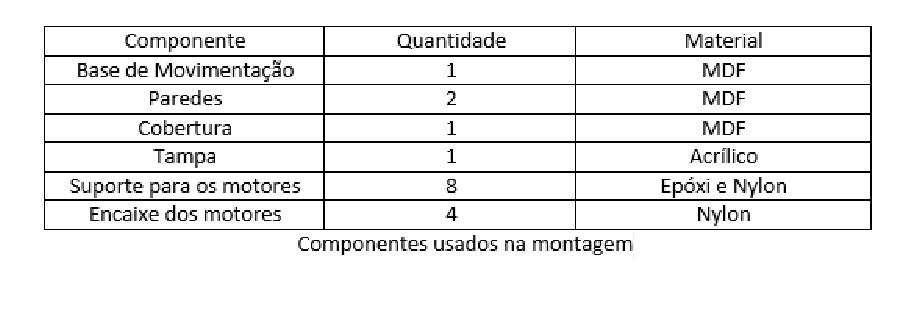
\includegraphics[width=1\textwidth]{figuras/usados.eps}
    \caption{Componentes usados na montagem}
    \label{fig:usados}
\end{figure}

A base de movimentação, as paredes e a cobertura foram construídas a partir de placas planas de MDF, onde utilizando algumas técnicas
de marcenaria conseguiu-se chegar à forma desejada. Devido ao método de fabricação das peças, canais foram criados na madeira, entretanto,
passado o processo de entalhe na madeira, tais canais se tornaram sem utilidade e fragilizaram a estrutura por um todo, para isso os canais
foram preenchidos com resina epóxi. Como se pode ver, há uma certa diferença da aparência final das peças feitas no CATIA e da real aparência
apresentada pelas peças, isso se deve as limitações físicas do processo empregado, e ao fato de todo o processo ter sido feito manualmente.

Alguns dos suportes para os motores e os encaixes, foram impressos utilizando uma impressora 3D da própria faculdade, os componentes também
não estão semelhantes aos projetados no CATIA devido a alguns problemas de calibragem na impressora, gerando nos componentes o chamado efeito
de borda. Alguns dos suportes foram conseguidos de uma outra estrutura e adaptado para uso no projeto.

Para a montagem final do carrinho os equipamentos eletrônicos, juntamente com a bateria e os motores e seus encaixes são fixados na base de
movimentação, após a fixação as paredes são coladas a base de movimentação e uma na outra, em camadas, e por último tem se a fixação da cobertura
e da tampa de acrílico (também coladas).

